% !TeX root = ../main.tex
% Add the above to each chapter to make compiling the PDF easier in some editors.

\chapter{Implementation}\label{chapter:implementation}

As explained in \autoref{sec:terminology}, from now on the term Firmware ID (FWID) will be used instead of the previously used term TCB Component Identifier (TCI).

\section{Overview}


We run our implementation on Arm's Fixed Virtual Platform~(FVP)\footnote{\url{https://developer.arm.com/Tools\%20and\%20Software/Fixed\%20Virtual\%20Platforms}} which is a complete simulation of the Armv8-A architecture including TrustZone.

To do this, we use the software infrastructure provided by OP-TEE for various platforms, including FVP\@.
OP-TEE uses the TrustedFirmware-A~(TF-A)\footnote{\url{https://www.trustedfirmware.org/projects/tf-a/}} package from Arm as firmware boot components.
However, we mock their attestation, i.e., their Alias certificates are statically compiled into the binaries instead of being dynamically generated, as TF-A does not implement DICE\@.
The development efforts to implement that exceeds the benefits, as the concept can also be demonstrated with mocked certificates.
For that, only the certificates up to the OP-TEE~OS are mocked, including OP-TEE~OS's private key to sign the subsequent Alias certificate, which is our EKcert.

Our implementation with compilation and running instructions can be found on GitHub.\footnote{\url{https://github.com/akorb/master-thesis-meta}}

\section{Boot chain}

The boot process is depicted in \autoref{fig:boot_chain}.
DICE is the root of trust, because incorrect behavior remains undetected and would jeopardize the security of our attestation process.

\begin{figure}[htpb]
  \centering
  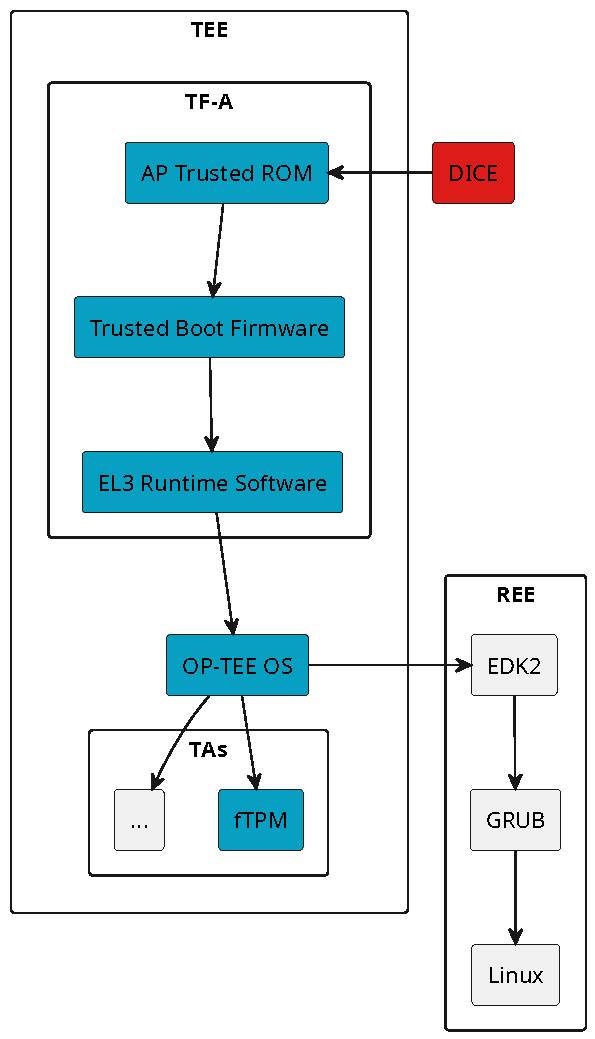
\includegraphics[width=0.8\linewidth]{figures/boot-chain.pdf}
  \caption{The boot chain of our system running in Arm's FVP\@. Blue: Represented by our yielding certificate chain. Red: Root of trust for verifier, and assumed to be present.}\label{fig:boot_chain}
\end{figure}



\paragraph{DICE}
Theoretically, the boot chain begins with the DICE hardware, but this is not included in FVP\@.
Therefore, we simply assume its presence by mocking the first few certificates of the yielding certificate chain.
Furthermore, it is independent hardware, and therefore, neither part of the TEE nor the REE\@.

\paragraph{TF-A}
After reset, the CPU executes within the secure world.
That is also the reason why machines that are unaware of the separation between secure world and normal world are running in the secure world, as they never modify the execution environment of the processor.
This also ensures that TrustZone unaware systems have all expected privileges, which would be restricted in the normal world.
The Application Processor~(AP) Trusted ROM sets up the platform-specific exception vectors.
The Trusted Boot Firmware enables the MMU, performs the platform security setup, and other tasks.
The final component of TF-A --- EL3 Runtime Software --- replaces the simple and rudimentary initialization performed by the AP Trusted ROM with more complete configurations by detecting the system topology, and enabling normal world software to function correctly.
The EL3 Runtime Software also provides the monitor which conducts the context switches between the secure world and the normal world.
More complete and detailed information can be found in the TF-A documentation.\footnote{\url{https://trustedfirmware-a.readthedocs.io/en/latest/design/firmware-design.html}}

\paragraph{OP-TEE~OS}
Finally, the OP-TEE~OS\footnote{\url{https://github.com/OP-TEE/optee_os}} is loaded and executed.
Just like an ordinary operating system, it initializes its functions offered to the user space of the secure world, i.e., the trusted applications.

\paragraph{Trusted Applications}

Our TA in focus is the firmware TPM\@.\footnote{\url{https://github.com/microsoft/ms-tpm-20-ref/}}
It consists of the reference code by Microsoft which implements a TPM, and the stub code, which provides and implements the interfaces required to be a TA of OP-TEE\@.
This fTPM only allows a single connection at any time, i.e., it prohibits concurrent access as this could lead to inconsistent states.
This also mirrors hardware TPMs, which are usually attached via serial buses like SPI to the processor.
Typically, the only entity that communicates with the fTPM is a Linux kernel module\footnote{\url{https://docs.kernel.org/security/tpm/tpm_ftpm_tee.html}}, so it is transparent to the user applications whether the TPM is implemented in firmware or hardware.
Note that TAs are not started automatically.
In fact, we are not aware of any function provided by OP-TEE~OS to register a TA to be started during the boot process. 
Instead, TAs are initialized the first time someone wants to interact with them.

\paragraph{EDK2}
TianoCore EDK II\footnote{\url{https://github.com/tianocore/edk2}} is the first component launched in the normal world.
It is a reference implementation of UEFI~\cite{UEFI} by Intel.

\paragraph{GRUB}
The GNU GRand Unified Bootloader\footnote{\url{https://www.gnu.org/software/grub/}} is a bootloader which is responsible for loading and transferring control to OS kernel software.

\paragraph{Linux}
As expected, the final component to boot is the Linux\footnote{\url{https://www.kernel.org/}} operating system.

\section{Firmware TPM initialization}

Initialization begins with the derivation of all secrets from the CDI\@.
Note that we mocked the CDI that would be passed from OP-TEE OS to the fTPM in practice.
However, OP-TEE OS does not implement DICE\@.

We use the Mbed TLS library\footnote{\url{https://mbed-tls.readthedocs.io/en/latest/}} providing cryptographic primitives for the derivation of the secrets, and also to build X.509 certificates.
Mbed TLS is already part of OP-TEE, and its functionality is modular and allows certain functionality to be activated or deactivated at a fine granular level.
Since the target machines are embedded devices with limited resources, the user should only activate the functions that he really needs.
We therefore had to activate some functions.

The formulas which derive secrets directly from the CDI (\autoref{eq:storage_key_formula}, \autoref{eq:eps_formula}) use a keyed-hash message authentication code~(HMAC) function.
This is inspired by the CDI derivation proposed in the DICE hardware requirements specification~\cite{dice-hardware-reqs}.
Actually, it proposes two functions to combine information to a new secret.
A simple hash function, and the HMAC function.
It also states that it recommends the HMAC function which calculation takes a little more time, but protects the CDI with twice the level than the simple hash function.
% https://nvlpubs.nist.gov/nistpubs/SpecialPublications/NIST.SP.800-57pt1r5.pdf (Table 3) shows that the HMAC version has roughly double security strength
This is backed by Jäger et al.~\cite{Jaeger2017}, and NIST SP 800--57~\cite{Barker2020}.
We declare the inner hash function used by the HMAC according to the required data size of the secret.
For example, for storage encryption, we use AES-256, and therefore, use the SHA256 function to retrieve a key with a sufficient size.
The HMAC functions are seeded with a fixed character string that describes the purpose of the output secret, e.g., `EPS'.

% Formula from (2) in https://trustedcomputinggroup.org/wp-content/uploads/Hardware-Requirements-for-Device-Identifier-Composition-Engine-r78_For-Publication.pdf
\begin{align}
  \label{eq:storage_key_formula}
  K_{storage} &= HMAC_{SHA256}(CDI,\ `DATA\ STORAGE\ KEY\text{'})\\
  \label{eq:eps_formula}
  EPS &= HMAC_{SHA512}(CDI,\ `EPS\text{'})\\
  \label{eq:ek_formula}
  EK  &= KDF(EPS,\ EK_{template})
\end{align}

\begin{figure}[htb]
  \centering
  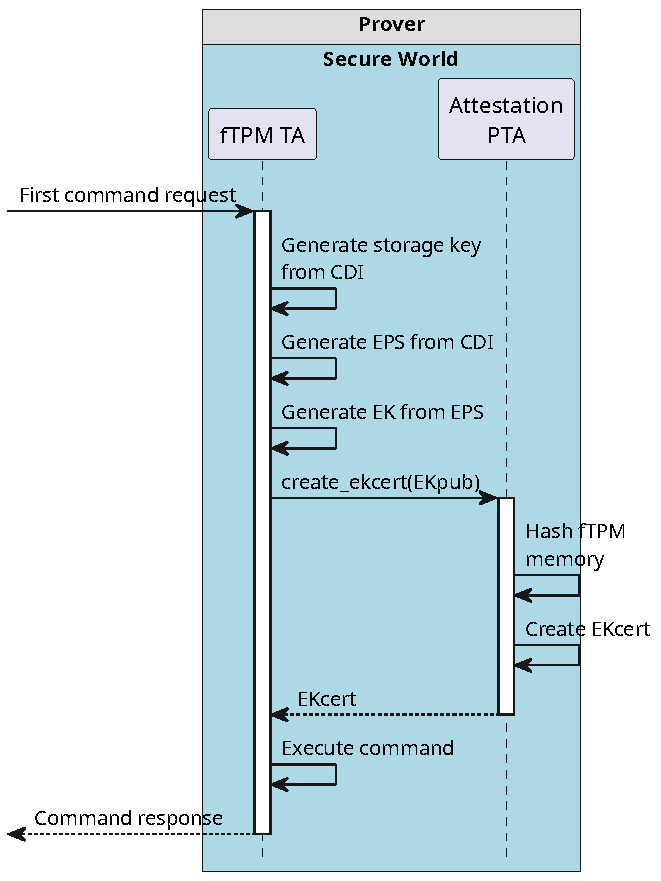
\includegraphics[width=0.62\linewidth]{figures/tpm-initialization.pdf}
  \caption{A UML sequence diagram describing the initialization of our firmware TPM\@.}\label{fig:ftpm_initialization}
\end{figure}


We must ensure we retrieve exactly the same EK as the TPM would generate by a \texttt{TPM2\_CreatePrimary} command with our EK template.
Therefore, we use the TPM internal functions to generate the EK\@.
The EK consists of a private and a public portion.
The private part never leaves the TPM, and the public portion is forwarded to OP-TEE's attestation PTA to be used as the subject key for EKcert, as shown by \autoref{fig:ftpm_initialization}.
A pseudo trusted application~(PTA) provides the same interfaces as an ordinary TA, with the difference that it does not run in user mode of the secure world, but in kernel mode within OP-TEE~OS\@.
Therefore, it has more privileges than an ordinary TA\@.
The attestation PTA requires these privileges in order to read the memory of the calling TA, i.e., the fTPM TA, which is processed into the FWID that is finally embedded in the EKcert.
The attestation PTA signs EKcert with OP-TEE's private alias key.
This key is mocked in our implementation.
Note that the fTPM has never access to the private alias key of OP-TEE OS, so it cannot spoof its alias certificate/EKcert.

The attestation PTA hashes the memory pages of the calling TA that are executable or read-only data, i.e., are constant.
It can also simply extract the hash embedded in the TA's binary header.
A TA is an ELF binary wrapped in an OP-TEE specific format, which header contains a signature over all metadata and the payload, i.e., the ELF executable.
While it is simpler and faster, it does not attest the TA's dynamically linked libraries.
Although the reference firmware TPM does not link dynamically to any library, we use the attestation of the memory data to be more future-proof.

To embed the FWID into the EKcert, we use the X.509 extension defined by the DICE Attestation Architecture~\cite{TCGAttestation2021}.
Therein, the TCB Info Evidence Extension is defined.
It allows many FWIDs to be embed into an X.509 certificate.
Our implementation always only stores one FWID into each Alias certificate or EKcert.
However, the privacy focused architecture explained in \autoref{sec:privacy} could leverage the possibility to store multiple FWIDs in the extension.
Each FWID consists of an identifier of the hash algorithm used, and the according digest.
We use SHA256.
The TCB Info Evidence Extension is defined formally in the ASN.1 description language.
Consequently, we use ASN1c\footnote{\url{https://github.com/vlm/asn1c}} to translate this formal definition to C~code.
In particular, we use a self-compiled version of ASN1c, since its last official release dates back to 2017, whereby its generated C~code throws various warnings with a modern C~compiler.

The resulting certificate generated by the attestation PTA is returned to the firmware TPM, which also has access to all preceding certificates.
In our implementation, these preceding certificates are simply mocked.

\section{Firmware TPM attestation}\label{sec:impl_ftpm_attestation}

\begin{figure}[htb]
  \centering
  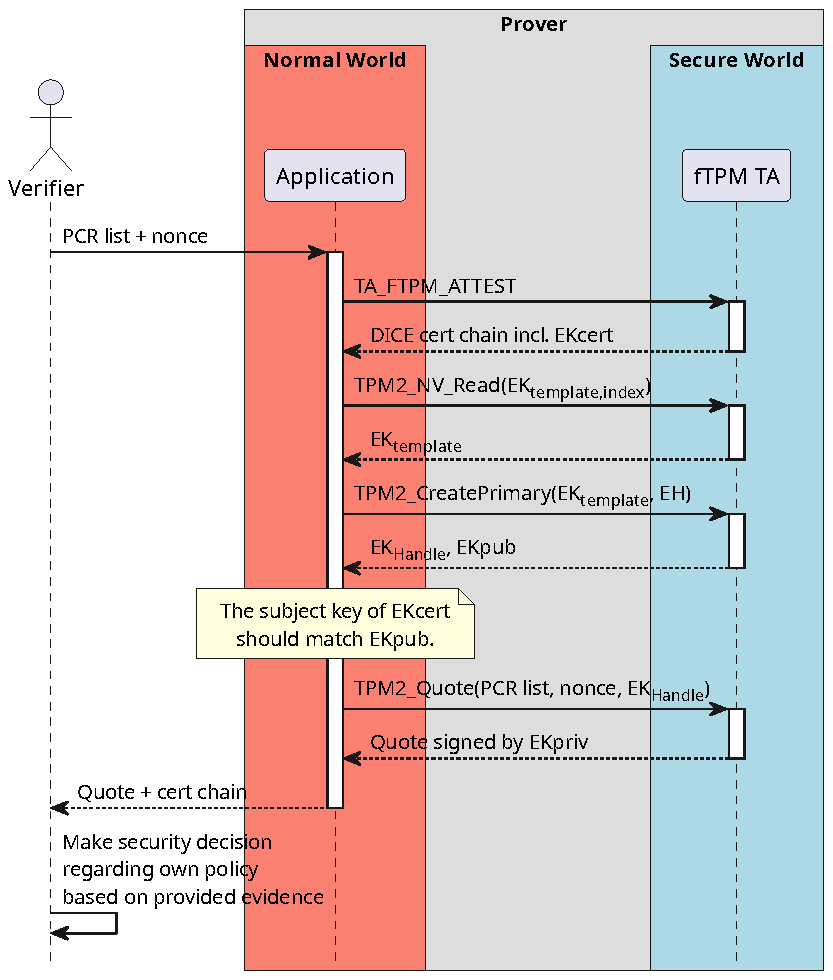
\includegraphics[width=0.74\linewidth]{figures/tpm-attestation.pdf}
  \caption{A UML sequence diagram describing the attestation of our firmware TPM\@.}\label{fig:ftpm_attestation}
\end{figure}


We added a new TA command called \texttt{TA\_FTPM\_ATTEST} to the firmware TPM to obtain the entire certificate chain from any application.
Normally, this command is issued by the application that performs the prover part of the remote attestation.
We would like to emphasize that we do not refer to a new TPM command that would imply an extension of the TPM specification, but a new TA command that is intercepted by the OP-TEE stub code of the fTPM and processed without the involvement of the TPM-specific core code.

Recall that we earlier described that the firmware TPM TA only ever allows a single connection to it, which is usually a Linux module that provide the \texttt{/dev/tpm0} and \texttt{/dev/tpmrm0} nodes to communicate with the fTPM\@.
We have therefore implemented the prover's side of the remote attestation with the ability to unload this Linux module before issuing \texttt{TA\_FTPM\_ATTEST}, and then load the Linux module again.

The prover's user space application starts with issuing the \texttt{TA\_FTPM\_ATTEST} command to the firmware TPM, as shown by \autoref{fig:ftpm_attestation}.
Consequently, it receives the certificate chain created by DICE with the EKcert as leaf certificate.

Afterwards, the prover wants the TPM to create the EK including its private portion.
To do this, it first reads the EK template from the non-volatile~(NV) memory of the fTPM, which was also used to create the EK part of the EK certificate.

Consequently, it then sends the template that has just been retrieved back to the TPM as part of the command \texttt{TPM2\_CreatePrimary}.
Since this command creates a primary key, no parent has be specified as the primary seed of the specified hierarchy is used instead.
Of course, we specify the endorsement hierarchy~(EH), which makes the TPM use the endorsement primary seed~(EPS) derived from the CDI to generate the EK\@.
The TPM returns a handle to the EK just created, which is an integer, as well as the public part of the EK\@.
The private part of the EK is not returned, as this never leaves the TPM in plain text.

Eventually, the prover wants to create a quote to establish trust to the prover's system state in the normal world, and to prove that it is in control of the EKpriv.
So, it issues the command \texttt{tpm2\_quote} to the TPM, specifying the PCR registers requested by the verifier, the verifier supplied nonce, and the handle to the EK just generated.

The prover's application handling the remote attestation is now in possession of the certificate chain, and a quote.
It transmits both to the verifier.
The verifier extracts the EKpub which is the subject key of the EKcert.
With that, it can verify the digital signature of the quote.
The ability of creating a quote with a fresh nonce proves the control of EKpriv by the fTPM\@.
Therefore, the verifier can trust that the certificate chain does not have been replayed, and it represents the device it communicates with.

In our implementation of the prover we do not send the TPM commands to the TPM ourselves, but use \texttt{tpm2\_createek~-t} and \texttt{tpm2\_quote} from the tpm2-tools.\footnote{\url{https://github.com/tpm2-software/tpm2-tools}}
Nevertheless, it executes these commands behind the scenes.
We also use \texttt{tpm2\_checkquote} in the verifier's implementation to check the signature of the quote, and to ensure that the nonce in the quote matches the nonce that the verifier has previously generated.

Note that the implementation just described assumes that the quote returned by \texttt{TPM2\_Quote} contains the values of the PCR registers.
While this was the case with TPM~1.2, this changed with version~2.0.
Instead, the resulting quote only contains a hash of the values of the requested PCR registers.
The corresponding plain text PCR values are transmitted unprotected to the verifier.
After validating the quote, the verifier can check whether the hash of the plain text PCR values computed by itself matches the PCR hash from the quote.
If this is the case, it can trust them.
This is also done by the tool \texttt{tpm2\_checkquote}.
We have omitted it from the previous explanation and \autoref{fig:ftpm_attestation} in order to focus on the important aspects.
For the sake of completeness and correctness, we mention it here anyway.

As a small note, we made sure that the property \texttt{tpmGeneratedEPS} of our fTPM is set to 1 as it indicates that the EPS was generated by the TPM~\cite{tpm}, which is the case in our implementation as it is derived from the CDI within the TPM\@.


\section{Creating and storing our EK template and certificate}
% \section{Adaption of the Endorsement Key}

The EK is a primary key, so it is derived from the EPS, and also a key template.
The template must be provided as part of the command \texttt{TPM2\_CreatePrimary} to the TPM\@.
The TPM can contain a template for an EK key, which shall be the template with which the EK part of the EKcert was created.
This is necessary to be able to reproduce the EK contained in the EK certificate so that the TPM can prove that this EK certificate corresponds to it by being able to generate the corresponding private key.

However, a TPM might not store an EK template.
Then, the default template defined by TCG~\cite{tcg-ek} is used, dictating the endorsement key to be a restricted encryption key, since it is privacy-sensitive, and that it must be an RSA~2048 key.
As this is fitting for most TPM's, the definition of the default template removes the burden of most TPM's to provide the template.
It is then the duty of the entity communicating with the TPM to provide the default EK template, since it is unknown to the TPM itself.
Though, we extended our firmware TPM to be able to generate the default and our custom EK template within code, such that it can create the EK which it forwards to the OP-TEE~OS to create the EK certificate.

% The default template is not stored on the TPM, but it is part of the command triggering the key generation (\texttt{TPM2\_CreatePrimary}).
% Therefore, the TPM itself does not need to know what the default template is, since it is always provided by TPM-capable software.

We want to use the EK as a signing key to sign attestation data, i.e., a quote.
Hence, we need to deviate from the default EK template, and also provide our template within the NV of our fTPM\@.
We start with the default EK template and only modify the fields when necessary.
In total, we needed to change three aspects.
We declare the EK as a (i)~restricted signing key.
This also requires to specify a (ii)~signature scheme where we selected RSASSA-PKCS1-v1\_5~\cite{Jonsson2003} with SHA-256, and (iii)~no inner symmetric key as required by the TPM specification~\cite{tpm} for signing keys since they are not allowed to have any children keys, as a signing key cannot encrypt its children for storage outside the TPM\@.

% We create this EK template within the firmware TPM in code on its first launch after any reset.
This template will be generated within the TPM after each manufacturer reset, so it will be preserved even after an identity change and a subsequent reset of the firmware TPM\@.
Thus, it is always present.
It is stored in the NV index \texttt{0x01c00004} as defined by the TPM EK specification~\cite{tcg-ek} for RSA 2048 EK templates.
We set the attributes for this NV index as defined by the TPM PC Client specification~\cite{tcgPcClient}. % 4.5.2.1
Thereby, the EK template in the NV can only be written or deleted if a specific policy is fulfilled.
However, the policy is empty, which can never be fulfilled.
This results in a non-deletable EK template.
We also store the EKcert in the NV index \texttt{0x01c00002} as defined by the TCG EK Credential Profile~\cite{tcg-ek} with the same attributes as the respective template.
The template and certificate do not contain any sensitive material and can hence be read by anyone using the command \texttt{TPM2\_NV\_Read}.

Nevertheless, our firmware TPM does not retrieve the EK template from the NV index to create the EK to subsequently forward it to the OP-TEE~OS to generate the EK certificate.
This would entail an indirection via the NV storage, which is not attested.
Instead, we explicitly use the EK template generated by code, which is attested via the fTPM's TCI\@.
% Ensure that the template generated by code is also directly used, instead of indirectly via unmeasured storages.
The NV storage is not attested as it is working data and not configuration data.
Hence, the fTPM's TCI would not only represent the fTPM's behavior, but also its stored data.
Since a TPM can store arbitrary data, this would explode the amount of TCI values that the verifier needs to know in order to derive the trustworthiness.
% However, the component right before the fTPM knows the fTPM's CDI, could generate the according symmetric key to decrypt the NV storage, and integrate the required NV values in the FWID\@.
% By baking the EK template generation in code which is already attested (and the code exists anyways), we prevent this complexity.

% The working data is not attested, since this would restrict the functionality of the fTPM\@.
% So, the an NV index is with ordinary TPM commands, providing the required policy/authentication is fulfilled.
% We consider this configuration as out-of-scope for attestation, for the former mentioned reason.
% In other words, it could be that everyone can change the NV index, where the template is stored.
% And in the subsequent boot, we would create a EKcert for it, without anything.
% Therefore, during EKcert creation, generate the template in code (which is attested), and use this directly.


\section{Times in certificates and systems}

In \autoref{tab:cert_comparison} we presented the restrictions the Alias and the EK certificate specifications conduct on the valid times of the certificates.
Thereby, the period of validity of our certificates must be from a known time in the recent past, e.g., the component's build time, without expiration date.

We initially aimed for using the build time for the start of the validity period.
However, this turned out to be infeasible, since the guest machine in the FVP does not have internet access out of the box, and FVP also does not provide an option to use the time of the host.
Therefore, the time of the host and the FVP guest would need to be synchronized manually, requiring unnecessary engineering effort.
Instead, we fix the times of all entities, i.e., the guest machine and the certificate's validity periods.
This ensures that the FVP does not have to be configured for internet access which keeps the effort to launch the demonstration low, and results in a higher stability of the demonstration system.

We use \texttt{2023--07--25 00:00:00} as the start period for the certificates.
This date has no further meaning and was chosen arbitrarily at some point during development.
As required in the specifications, we indicate that the certificates do not have a well-defined expiration date, which is indicated by \texttt{9999--12--31 23:59:59}~\cite{Boeyen2008}.

The time of the guest machine is automatically set to \texttt{2023--08--02 11:46} with the Linux tool \texttt{date} at startup.
As before, this date has no further meaning.
It is only important that this date is after the start period of the certificates.

\section{Implementing encrypted storage}

Overall, the reference TPM's memory size has a size of 16896 bytes, separated in a NV storage of 16384 bytes, and the admin space of 512 bytes.
The admin space is reserved to persist defined data like the TPM's attributes, e.g., \texttt{tpmGeneratedEPS}.
The NV storage can store arbitrary data, e.g., the EK template, certificate, or an encryption key.
For example, Microsoft's BitLocker stores the encryption key for hard disk encryption in the NV storage.

The OP-TEE~OS manages storage in blocks.
It is only possible to write entire blocks, not partial blocks.
Therefore, little changes can be expensive to persist if the according block is big.
Hence, the OP-TEE specific code of the reference fTPM splits the memory size of 16896 bytes in 512 bytes blocks resulting in \( 16896 \div 512 = 33 \) blocks.

We use the recommendations of the BSI~\cite{bsi-key-recommendations} to determine the encryption method.
Therefore, we use AES-128 in GCM mode to protect the data's confidentiality and integrity with an initialization vector~(IV) and tags of length 96 bits.
These are the recommended minimum sizes that we have chosen in order to spare resources.
There is one IV and tag for each block, which results in a storage overhead of 792 bytes as shown in \autoref{eq:memory_overhead}.

\begin{equation}
  \label{eq:memory_overhead}
  \frac{33 \times (96 + 96)\ \text{bits}}{8} = 792\ \text{bytes}
\end{equation}

The IVs are randomized on every write event.
On any mismatch between the stored tag and the tag produced during decryption, the firmware TPM is reset. 

The data is loaded from the hard disk and then decrypted only at startup time.
And it is written only during shutdown of the TPM or if a command modifies the TPM's storage.
As data is mainly written to the TPM during the provisioning time and only read during daily use, we assume that the impact on performance will be small.

\section{Isolating storage of fTPM in OP-TEE}

The data of the individual TAs must be saved somewhere permanently, otherwise they would be lost after each restart.
This data must be protected as it is stored in OP-TEE in the REE\@ file system.
OP-TEE encrypts the secure storage files before sending them to the REE for permanent storage using a pseudo-randomly generated key, the File Encryption Key~(FEK).
It is stored in the metadata of the corresponding file, encrypted with a key unique to each trusted application, the Trusted Application Storage Key~(TSK). % (https://optee.readthedocs.io/en/latest/architecture/secure\_storage.html#trusted-application-storage-key-tsk).
It is derived from the Secure Storage Key~(SSK), which is unique to the device.
% \begin{itemize}
%   \item SSK:\ Unique per device
%   \item TSK:\ Unique per TA
%   \item FEK:\ Unique per file
% \end{itemize}
\begin{align}
  % \label{eq:ssk_formula}
  % SSK &= HMAC_{SHA256}(HUK,\ Chip\ ID\ \|\ `static\ string\text{'})\\
  \label{eq:tsk_formula}
  TSK &= HMAC_{SHA256}(SSK,\ TA_{UUID})\\
  \label{eq:fek_formula}
  FEK &= decrypt_{TSK}(File_{metadata})\\
  data_{plain} &= decrypt_{FEK}(File_{payload})
\end{align}
% where HUK is a hardware unique key, and the chip ID a UUID unique to the hardware, possibly derived from the HUK\@.
% More details can be found in OP-TEE's documentation\footnote{\url{https://optee.readthedocs.io/en/latest/architecture/porting\_guidelines.html}}.

\autoref{eq:tsk_formula} shows that the TSK depends only on the SSK and the TA's UUID\@.
As said, the SSK is same for the whole device and hence for every TA, and the \( TA_{UUID} \) is public.
A close look reveals that other TA's on the same device could therefore use the publicly available UUID to generate the fTPM's TSK and consequently, decrypt the FEKs of the fTPM's files and access private data of the fTPM\@.
However, this is prevented by our integration of an additional storage key, which encrypts the data before it is sent to the OP-TEE~OS\@.

The TEE specification offers an ultimate solution for that on the conception level of the trusted OS without requiring a manual encryption step in the TA itself.
It is defined in the TEE Management Framework~\cite{GP_ManagementFramework}, which offers the possibility of grouping TAs into domains and subdomains, whereby only TAs in the same domain or subdomain can potentially decrypt each other's data.
However, as of time of writing, this is not implemented in OP-TEE~OS yet.

\section{Technical obstacles}

\subsection{tpm2-tools}

As mentioned earlier, we use the \texttt{tpm2\_checkquote} tool to verify the prover's quote on the verifier's side.
However, this tool fails to perform an important check to ensure that the quote was generated by the TPM and not externally.
This poses a major security risk.
We have reported this to the authors of the tpm2-tools via the recommended channel.\footnote{\url{https://github.com/tpm2-software/tpm2-tools/security/advisories/GHSA-5495-c38w-gr6f}}

% \paragraph{RSASSA-PSS vs. RSASSA-PKCS1-v1\_5}
We would have liked to use RSASSA-PSS which is formally proven to be secure over RSASSA-PKCS1-v1\_5.
RFC 8017 even requires RSASSA-PSS for new applications~\cite{Moriarty2016}.
However, it is not fully supported by the tpm2-tools, yet.\footnote{\url{https://github.com/tpm2-software/tpm2-tools/issues/3283}}

The tool \texttt{tpm2\_createek} did not adhere to the TPM specification when it created the EK with a template from the NV storage of the TPM\@.
A template always contains a nonce, but it can be overwritten by storing another nonce in a specifically defined NV index.
We did not want to deviate from the standard nonce, which is a buffer of 256\,bytes all set to 0.
Therefore, we did not write a nonce to the NV index, and only the EK template with the default nonce, which conforms to the TPM specification~\cite{tcg-ek}.
However, \texttt{tpm2\_createek} expected a template and a nonce to be present.
We ended up writing an empty nonce in the according NV index of the firmware TPM with the sole aim of circumventing this problem.
Then, it turned out that this tool has another bug that caused the address of the nonce  to be used instead of the actual nonce.
We have fixed this bug.\footnote{\url{https://github.com/tpm2-software/tpm2-tools/pull/3280}}


\subsection{OP-TEE}

% Build

Initially, it failed to follow the official documentation to create the complete software ecosystem with the reference firmware TPM enabled.
Eventually, we determined the problem and fixed it.\footnote{\url{https://github.com/OP-TEE/optee_os/issues/6111}}

% Persistence

It was important for us to also test whether our system behaves as expected if the CDI changes.
For that, we needed to persist the storage of the firmware TPM between launches of the FVP to modify the CDI during its downtime.
However, the FVP version required to accomplish this turned out to freeze when the necessary functionality was activated.
It took extensive debugging efforts to find a workaround.\footnote{\url{https://github.com/OP-TEE/optee_os/issues/6162}}

The OP-TEE~OS provides a libc library which implements only subset of the C standard library.
Its authors copy code of the newlib\footnote{\url{https://sourceware.org/newlib/}} to their libc library on-demand when required.
Unfortunatley, the code generated by the asn1c project expects functions not part of OP-TEE's libc.
Fortunately, these functions were not critical and could be removed manually in a reasonable amount of time.

\subsection{Firmware TPM TA}

We have enabled a compilation option offered by the fTPM TA which appears not to have been thoroughly tested.
When the option is enabled, the TPM uses code written specifically to use the OP-TEE functions to generate the EPS\@.
This resulted in a crash of the fTPM during startup.
We fixed the bug and opened a pull request for the fix to be merged upstream.\footnote{\url{https://github.com/microsoft/ms-tpm-20-ref/pull/98}}

Eventually, we did not use this code.
Nevertheless, this bug was found in the context of this thesis, and hence, we want to mention it here.
